%%%%%%%%%%%%%%%%%%%%%%%%%%%%%%%%%%%%%%%%%%%%%%%%%%%%%%%%%%%%%%%%%%%%%%
\begin{frame}[fragile]\frametitle{}
\begin{center}
{\Large Maps}
\end{center}

\end{frame}

%%%%%%%%%%%%%%%%%%%%%%%%%%%%%%%%%%%%%%%%%%%%%%%%%%%%%%%%%%%%%%%%%%%%%%
\begin{frame}
	\frametitle{The map ADT}
	
Maps work on \textit{key-value} pairs, usually denoted as tuples: $(k,v)$.
			
			\begin{itemize}
				\item \texttt{M.size()} (or \texttt{len(M)}) to get the number of tuples in the map.
					
				\item \texttt{M.get(k)} (or \texttt{M[k]}) to retrieve the value for key $k$.
				\item \texttt{M.put(k,v)} (or \texttt{M[k] = v}) to set the value for key $k$ to $v$.
					
				\item \texttt{M.remove(k)} (or \texttt{del M[k]}) to remove the tuple with key $k$.
					
				\item \texttt{M.contains(k)} (or \texttt{k in M}) to determine if there is tuple with key $k$.
			\end{itemize}

\end{frame}

%%%%%%%%%%%%%%%%%%%%%%%%%%%%%%%%%%%%%%%%%%%%%%%%%%%%%%%%%%%%%%%%%%%%%%
\begin{frame}
	\frametitle{A naive implementation: Listing a map}

			\begin{itemize}
				\item Why not just use a list?: If we use a list to implement the map where we just throw in all the tuples, what would the time complexity
		of the functions \texttt{get}, \texttt{remove}, \texttt{contains} be?
						\item Which?
		\begin{itemize}
			\item $\Theta(1)$
			\item $\Theta(\log n)$
			\item $\Theta(n)$
			\item $\Theta(n^2)$
			\item I don't know
		\end{itemize}
		
				\item Not so great:		All would take linear time! 
 				\item We would just have to check all the objects every time!
	\end{itemize}
\end{frame}

%%%%%%%%%%%%%%%%%%%%%%%%%%%%%%%%%%%%%%%%%%%%%%%%%%%%%%%%%%%%%%%%%%%%%%
\begin{frame}
	\frametitle{Can we do better?}
		\begin{itemize}
			\item Can we do better, and if so how?
			\item How about we try to use an array-based structure where the key determines the index?
			\item This allows for $\Theta(1)$ operations for getting, removing or checking an item!
			\item But what if the key is not integer?
	\end{itemize}
\end{frame}

%%%%%%%%%%%%%%%%%%%%%%%%%%%%%%%%%%%%%%%%%%%%%%%%%%%%%%%%%%%%%%%%%%%%%%
\begin{frame}
	\frametitle{Hash functions}
	
		\begin{itemize}
			\item Hash functions map each key $k$ to a an integer in a range $[0, N-1]$ for some $N$.
			\item Consider the hash function $f(k) = 1$ for any key $k$.
			Is this a hash function for $N=100$?
			\begin{itemize}
				\item Yes
				\item No
				\item I don't know
			\end{itemize}
			\item It is a hash function, but a terrible one!
				Why?
		\end{itemize}	
\end{frame}

%%%%%%%%%%%%%%%%%%%%%%%%%%%%%%%%%%%%%%%%%%%%%%%%%%%%%%%%%%%%%%%%%%%%%
\begin{frame}
	\frametitle{Hash to determine the index}

		\begin{itemize}
			\item We want to use hash functions to map keys to a certain index in a hash table.
			\item Back to hundred-acre woods:
		Take $f(p) = 1$, $f(i) = 3$, $f(g) = 2$, $f(l) = 8$, $f(e) = 5$, $f(t) = 7$.
		
			\item This would create the hash table:
		\begin{center}
			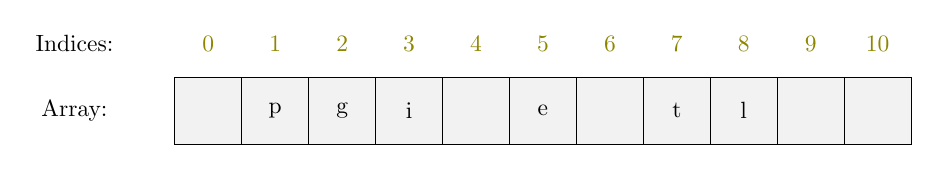
\begin{tikzpicture}[scale=0.85, transform shape]
	\foreach \x/\val in {0/,1/p,2/g,3/i,4/,5/e,6/,7/t,8/l,9/,10/}{
	\node[olive] (index) at (\x,1) {\x};
	\node[draw,rectangle, fill=gray!10, minimum size =1cm] (c) at (\x,0) {\val};
}
\node[] at (-2,1) {Indices:};
\node[] at (-2,0) {Array:};
\end{tikzpicture}

		\end{center}
\item The simple mapping:
		But what if we have conflicts? Like by taking $f(k)=1$ for all $k$.
	\end{itemize}	
\end{frame}

%%%%%%%%%%%%%%%%%%%%%%%%%%%%%%%%%%%%%%%%%%%%%%%%%%%%%%%%%%%%%%%%%%%%%
\begin{frame}
	\frametitle{Hashing conflicts}

		\begin{itemize}
			\item We want to use hash functions to map keys to a certain index in a hash table.\\
		But what do we do if we have hashing conflicts?
			\item Back to hundred-acre woods:
		Take $f(e) = 1$, $f(y) = 3$, $f(o) = \alert{3}$, $f(r) = 8$.
		
			\item This would create the hash table:
		\begin{center}
			\begin{tikzpicture}[scale=0.85, transform shape]
	\foreach \x/\val in {0/,1/,2/,3/,4/,5/,6/,7/,8/,9/,10/}{
	\node[olive] (index) at (\x,1) {\x};
	\node[draw,rectangle, fill=gray!10, minimum size =1cm] (\x) at (\x,0) {\val};
}
\node[] at (-2,1) {Indices:};
\node[] at (-2,0) {Array:};

\node[draw,rectangle, fill=gray!10, minimum size =0.5cm] at (1,-1.5) (e) {e};
\node[draw,rectangle, fill=gray!10, minimum size =0.5cm] at (3,-1.5) (A) {y};
\node[draw,rectangle, fill=gray!10, minimum size =0.5cm] at (3,-2.5) (B){o};
\node[draw,rectangle, fill=gray!10, minimum size =0.5cm] at (8,-1.5) (r) {r};
\draw[->, ultra thick] (A) -- (B);
\draw[*->, ultra thick] (1.center) -- (e);
\draw[*->, ultra thick] (3.center) -- (A);
\draw[*->, ultra thick] (8.center) -- (r);
\end{tikzpicture}

		\end{center}
	\end{itemize}	
\end{frame}

%%%%%%%%%%%%%%%%%%%%%%%%%%%%%%%%%%%%%%%%%%%%%%%%%%%%%%%%%%%%%%%%%%%%%
\begin{frame}
	\frametitle{Hash tables}
		\begin{itemize}
			\item We have an array of a certain capacity.
		The hash of a key, determines which \textit{bucket} to use.
			\item Every entry could for instance hold a linked-list of values.
			\item What happens?:
		So for $f(k) = 1$ for all $k$, what is the time complexity of getting the right value out for our key?
		\begin{itemize}
			\item $\Theta(1)$
			\item $\Theta(\log n)$
			\item $\Theta(n)$
			\item $\Theta(n^2)$
		\end{itemize}
			\item It is still linear time! All end up in a list after all.
		\end{itemize}
\end{frame}

%%%%%%%%%%%%%%%%%%%%%%%%%%%%%%%%%%%%%%%%%%%%%%%%%%%%%%%%%%%%%%%%%%%%%
\begin{frame}
	\frametitle{Hash functions: Ideal properties}
	
		\begin{itemize}
			\item Hash functions map each key $k$ to a an integer in a range $[0, N-1]$ for some $N$.
			\item Where ideally:
			
			\begin{itemize}
				\item keys are uniformly distributed over the range.
					
				\item ($a == b) \to (\mathit{hash}(a) == \mathit{hash}(b))$ (it is deterministic).
					
				\item the hash function is `fast' to compute (preferably $O(1)$).
			\end{itemize}
			\item This indeed makes $f(k) = 1$ pretty terrible!
			\end{itemize}	
\end{frame}

%%%%%%%%%%%%%%%%%%%%%%%%%%%%%%%%%%%%%%%%%%%%%%%%%%%%%%%%%%%%%%%%%%%%%
\begin{frame}
	\frametitle{Implementing them in Python}

	Which is better?	
			\begin{itemize}
			\item The left one.
			\item The right one.
			\item I don't know.
		\end{itemize}
		
			It depends on what kind of points we expect to see!

		
			\begin{itemize}
			\item \lstinputlisting{src/point.py}
			\item 
			\item \lstinputlisting[firstline=4, lastline=15]{src/point2.py}
	\end{itemize}
	


		
\end{frame}

%%%%%%%%%%%%%%%%%%%%%%%%%%%%%%%%%%%%%%%%%%%%%%%%%%%%%%%%%%%%%%%%%%%%%
\begin{frame}
	\frametitle{Hashmaps}
			\begin{itemize}
			\item Implement the Map ADT using Hash tables.
			\item With a good hash function, we expect: $\Theta(1)$ insertion/deletion/retrieval.
			But worst-case they are still $\Theta(n)$.
			\item Different options to handle hash conflicts:
			\begin{itemize}
				\item Separate Chaining
				\item (Linear) Probing
			\end{itemize}
		\end{itemize}
\end{frame}

%%%%%%%%%%%%%%%%%%%%%%%%%%%%%%%%%%%%%%%%%%%%%%%%%%%%%%%%%%%%%%%%%%%%%
\begin{frame}
	\frametitle{Lets start with the basics}
	\begin{columns}[T]
		\column{0.355\linewidth}
		\begin{itemize}
			\item Creating a new hashmap
			\item Getting the size
			\item A hash function for keys in this map
			\item Getting an item
			\item Putting an item
		\end{itemize}
		So conclusion: It depends on how we put things into the buckets!\\
				Do we use the linked list? Or do we do something else?
		\column{0.555\linewidth}
		\lstinputlisting[basicstyle=\tiny\ttfamily]{src/hashmap.py}
	\end{columns}
\end{frame}


%%%%%%%%%%%%%%%%%%%%%%%%%%%%%%%%%%%%%%%%%%%%%%%%%%%%%%%%%%%%%%%%%%%%%
\begin{frame}
	\frametitle{Recap of Maps}
	
	\begin{center}
		\begin{tabular}{c | c | c}
			Operation & Expected Time & Worst-case \\
			\midrule
			\texttt{M.size()} & $\Theta(1)$& $\Theta(1)$\\
			\texttt{M.get(k)}  & $\Theta(1)$& $\Theta(n)$\\
			\texttt{M.put(k,v)} & $\Theta(1)$& $\Theta(n)$\\
			\texttt{M.remove(k)} & $\Theta(1)$& $\Theta(n)$\\
			\texttt{M.contains(k)} & $\Theta(1)$& $\Theta(n)$\\
		\end{tabular}
	\end{center}
	
What does this depend on?:	It all stands or falls with the hash function!
			\begin{itemize}
				\item Fewer hash-conflicts means better performance.
				\item Separate chaining or (linear) probing does not matter for time performance.
				\item The latter saves us some space, but is not better in terms of space or time \textit{complexity}.
			\end{itemize}
\end{frame}

